% =====================================================================
% research-review standard Beamer preamble  (XeLaTeX, 16:9, slate-blue)
% Build: make slide PAPER=tcf-ehr   (XeLaTeX 2-pass, out-of-tree → build/)
% =====================================================================
\documentclass[10pt, aspectratio=169, t]{beamer}   % t: top-align frame bodies

% --- Theme (clean, no external theme packages) -----------------------
\usetheme{default}
\usecolortheme{default}
\useinnertheme{circles}
\setbeamertemplate{navigation symbols}{}

% --- Fonts: XeLaTeX + fontspec, sans-serif body ----------------------
\usepackage{fontspec}
\usefonttheme{professionalfonts}      % keep math glyphs in CM, not sans
\renewcommand{\familydefault}{\sfdefault}   % Latin Modern Sans body

% --- Packages --------------------------------------------------------
\usepackage{xcolor}
\usepackage{graphicx}
\usepackage{amsmath}
\usepackage{amssymb}
\usepackage{mathrsfs}
\usepackage{booktabs}
\usepackage{array}
\usepackage{colortbl}                 % \rowcolor for table row highlight
\usepackage[font=scriptsize]{caption}
\usepackage[most]{tcolorbox}
\usepackage{tikz}
\usetikzlibrary{arrows.meta, positioning}
\usepackage{pifont}                   % \ding checkmarks/crosses for Table 1

% --- Palette (3-5 colors, WCAG AA contrast) --------------------------
\definecolor{accent}{HTML}{1F3A5F}      % deep slate-blue — titles, rules, links
\definecolor{accentSoft}{HTML}{5C7AA0}  % muted slate — subtitles
\definecolor{ink}{HTML}{1A1A1A}         % body text
\definecolor{muted}{HTML}{6B6B6B}       % captions, metadata
\definecolor{rulec}{HTML}{D8DEE6}       % thin separator rules
\definecolor{boxbg}{HTML}{F4F6FA}       % tcolorbox / block background tint
\definecolor{crimson}{HTML}{780016}     % rare emphasis only (diagrams)
% --- Semantic keyword emphasis: positive = blue, negative = magenta --------
\definecolor{posblue}{HTML}{0066FF}     % positive-wording emphasis (blue)
\definecolor{negmag}{HTML}{D6009C}      % negative-wording emphasis (magenta)
\newcommand{\good}[1]{{\color{posblue}\bfseries #1}}  % wrap positive keyword
\newcommand{\warn}[1]{{\color{negmag}\bfseries #1}}   % wrap negative keyword
\newcommand{\blue}{\color{posblue}\bfseries}  % legacy switch -> positive (now bold)
\newcommand{\hl}{\color{posblue}\bfseries}    % legacy standout -> positive blue

% --- Beamer colors ---------------------------------------------------
\setbeamercolor{normal text}{fg=ink}
\setbeamercolor{structure}{fg=accent}
\setbeamercolor{frametitle}{fg=accent}
\setbeamercolor{framesubtitle}{fg=accentSoft}
\setbeamercolor{title}{fg=accent}
\setbeamercolor{subtitle}{fg=accentSoft}
\setbeamercolor{section in toc}{fg=accent}
\setbeamercolor{itemize item}{fg=accent}
\setbeamercolor{itemize subitem}{fg=accentSoft}
\setbeamercolor{enumerate item}{fg=accent}
\setbeamercolor{block title}{fg=white, bg=accent}
\setbeamercolor{block body}{fg=ink, bg=boxbg}
\setbeamercolor{caption name}{fg=accent}

\setbeamerfont{frametitle}{series=\bfseries, size=\large}
\setbeamerfont{framesubtitle}{series=\mdseries, size=\small}
\setbeamerfont{title}{series=\bfseries, size=\LARGE}
\AtBeginDocument{\small}   % single body baseline for the whole deck

% --- Footline: short-title (left) / page (right) ---------------------
\setbeamertemplate{footline}{%
  \leavevmode%
  \hbox{%
    \begin{beamercolorbox}[wd=\paperwidth, ht=2.4ex, dp=1.5ex, leftskip=1.2em, rightskip=1.2em, sep=0pt]{}%
      {\color{muted}\scriptsize\insertshorttitle}%
      \hfill%
      {\color{accent}\scriptsize$\bullet$}\hspace{0.6em}%
      {\color{muted}\scriptsize\insertframenumber\,/\,\inserttotalframenumber}%
    \end{beamercolorbox}%
  }%
  \vspace{2pt}%
}

% --- Itemize bullets -------------------------------------------------
\setbeamertemplate{itemize item}{\small$\blacktriangleright$}
\setbeamertemplate{itemize subitem}{\small$\triangleright$}
\setbeamertemplate{itemize subsubitem}{\scriptsize\textendash}

% --- Section divider: one full-bleed page per section ----------------
\AtBeginSection[]{%
  \begin{frame}[plain, noframenumbering, c]
    \vfill
    \begin{center}
      {\color{muted}\scriptsize\MakeUppercase{Section \insertsectionnumber}}\\[8pt]
      {\color{accent}\Large\bfseries\insertsectionhead}\\[12pt]
      {\color{accent}\rule{0.22\paperwidth}{0.8pt}}
    \end{center}
    \vfill
  \end{frame}%
}

% --- tcolorbox defaults: inline title (box width = content width) ----
\tcbset{
  enhanced,
  colframe=accent!55,
  colback=boxbg,
  coltitle=accent,
  boxrule=0.4pt,
  arc=2pt,
  left=5pt, right=5pt, top=3pt, bottom=3pt,
  fonttitle=\bfseries\small,
  title style={left color=accent!8, right color=accent!8},
  separator sign={\,:},
}

\hypersetup{colorlinks=true, linkcolor=accent, citecolor=accent, urlcolor=accent}

\DeclareMathOperator*{\argmax}{argmax}
\DeclareMathOperator*{\argmin}{argmin}

% Small helper: muted caption line under a figure/table
\newcommand{\figcap}[1]{{\color{muted}\scriptsize #1}}

% =====================================================================
\title[TCF: EHR Foundation Model]{Time-Conditioned Foreseeing:\\ An EHR-Specific Foundation Model for\\ Irregular Dynamics and Calendrical Time}
\subtitle{Temporal Generative Pretraining for EHR Foundation Models \textperiodcentered{} ICML 2026}
\author[Research Review]{Research Review \quad\textbar\quad Presenter: Changhyun Park}
\date{2026.06.23}

\begin{document}

% ---------------------------------------------------------------------
% Title
% ---------------------------------------------------------------------
\begin{frame}[plain, noframenumbering, c]
  \titlepage
  \begin{center}
    \figcap{Bong Gyun Kang, Junyong Ahn, Hyeongrok Han, Sungroh Yoon \textperiodcentered{} Seoul National University \textperiodcentered{} ICML 2026}\\[5pt]
    {\color{accent}\scriptsize \textbf{Poster} \textperiodcentered{} Thu 9 Jul, 10:30--12:15 KST \textperiodcentered{} Hall A \#808 \textperiodcentered{} COEX, Seoul}
  \end{center}
\end{frame}

% ---------------------------------------------------------------------
% TL;DR
% ---------------------------------------------------------------------
\begin{frame}{TL;DR}
  \framesubtitle{EHRs are not natural language --- so stop training them like it}
  \vfill
  \begin{itemize}\setlength{\itemsep}{9pt}
    \item \textbf{Problem} --- EHR foundation models inherit NLP recipes: \warn{\emph{uniform binning, absolute positions, NTP/MLM}} --- ill-fit to EHR.
    \item \textbf{Idea} --- \good{three EHR-native designs}: \emph{Pathology-Focused Binning}, \emph{Dual-Calendar RoPE}, \emph{Time-Conditioned Foreseeing}.
    \item \textbf{Result} --- ranks \#1 on all 3 feature configs $\times$ 7 tasks \textperiodcentered{} AUPRC up to {\blue +48\%} vs.\ 2nd-best \textperiodcentered{} \good{realistic temporal generation}.
  \end{itemize}
  \vfill
  \begin{columns}[t]
    \begin{column}{0.5\textwidth}
      \begin{tcolorbox}[title={Contributions}]
        \begin{itemize}\setlength{\itemsep}{3pt}
          \item Density-based binning $\to$ \emph{pathologic} ranges
          \item RoPE split: position $\Vert$ \emph{calendrical} time
          \item TCF $=$ next-time $+$ multi-horizon foresee
        \end{itemize}
      \end{tcolorbox}
    \end{column}
    \begin{column}{0.5\textwidth}
      \begin{tcolorbox}[title={Headline}]
        First \emph{genuine} temporal generative EHR model\\[3pt]
        MIMIC-III \textperiodcentered{} 8 baselines \textperiodcentered{} 117/17/6 features\\[3pt]
        {\hl $\sim$50\%} AUPRC gain on decompensation tasks
      \end{tcolorbox}
    \end{column}
  \end{columns}
  \vfill
\end{frame}

% =====================================================================
\section{Motivation}
% =====================================================================

% ---------------------------------------------------------------------
% Motivation: EHR != NL
% ---------------------------------------------------------------------
\begin{frame}{EHRs are not natural language}
  \framesubtitle{NLP-paradigm EHR models discard exactly what makes EHR clinical}
  \vfill
  \begin{itemize}\setlength{\itemsep}{8pt}
    \item EHR event $=$ \textbf{(Time, Feature, Value)} triplet --- e.g.\ \emph{(14:04, SBP, 87\,mmHg)}.
    \item \emph{But} most models \warn{\textbf{drop Time or Value}} due to modeling complexity (Table 1).
    \item \textbf{Loosely-coupled events} --- neighbors weakly correlated; long-range deps (e.g.\ 8-h follow-up), \emph{unlike} grammar where one missing token breaks the sentence.
    \item \textbf{Irregular intervals} --- minutes vs.\ hours apart; NLP assumes \emph{uniform} spacing.
    \item \textbf{Numeric-dominant} --- pathologic ranges are rare yet clinically decisive.
  \end{itemize}
  \vfill
  \begin{tcolorbox}[title={Why it matters}]
    Borrowing NLP recipes wholesale $\Rightarrow$ \warn{\emph{suboptimal}} EHR models --- timing, severity, and calendrical context are all flattened away.
  \end{tcolorbox}
  \vfill
\end{frame}

% ---------------------------------------------------------------------
% Three inherited NLP mismatches
% ---------------------------------------------------------------------
\begin{frame}{Three inherited mismatches this paper fixes}
  \framesubtitle{Each NLP default fails a specific EHR property}
  \vfill
  \begin{center}
  \renewcommand{\arraystretch}{1.35}
  \setlength{\tabcolsep}{6pt}
  \begin{tabular}{@{}>{\raggedright\arraybackslash}p{0.20\textwidth} >{\raggedright\arraybackslash}p{0.34\textwidth} >{\raggedright\arraybackslash}p{0.37\textwidth}@{}}
    \toprule
    \textbf{NLP default} & \textbf{EHR failure} & \textbf{This paper}\\
    \midrule
    Uniform value binning & bins crowd \emph{normal} ranges; few bins for \emph{pathologic} severity & \textbf{Pathology-Focused Binning} (density-based)\\
    \rowcolor{accent!8}
    Absolute positional emb.\ & loses \emph{relative} intervals \& \emph{calendrical} context (day/night, weekday) & \textbf{Dual-Calendar RoPE}\\
    NTP / MLM objective & only $P(F_{\text{next}}\!\mid\! E_{\text{past}})$; blind to \emph{when} and \emph{long-range} & \textbf{Time-Conditioned Foreseeing}\\
    \bottomrule
  \end{tabular}
  \end{center}
  \vfill
  \begin{itemize}\setlength{\itemsep}{4pt}
    \item NTP \warn{cannot tell whether} an event occurs \emph{minutes} or \emph{hours} later --- \warn{urgent and routine collapse to one} ``next token.''
  \end{itemize}
  \vfill
\end{frame}

% =====================================================================
\section{Related Work}
% =====================================================================

% ---------------------------------------------------------------------
% Related work landscape (Table 1)
% ---------------------------------------------------------------------
\begin{frame}{Landscape of EHR foundation models}
  \framesubtitle{Table 1. Prior models cover only fragments of the (Time, Value, Objective) space}
  \vfill
  \begin{center}
  \scriptsize
  \renewcommand{\arraystretch}{1.12}
  \setlength{\tabcolsep}{4pt}
  \begin{tabular}{l cc cc ccc l}
    \toprule
    & \multicolumn{2}{c}{\textbf{Data use}} & \multicolumn{2}{c}{\textbf{Value binning}} & \multicolumn{3}{c}{\textbf{Time addressing}} & \\
    \cmidrule(lr){2-3}\cmidrule(lr){4-5}\cmidrule(lr){6-8}
    \textbf{Model} & Time & Value & Non-unif. & Share & Rel.\ int. & Calend. & Non-conc. & \textbf{Objective}\\
    \midrule
    BEHRT / Med-BERT     & \ding{55} & \ding{55} & --       & --       & \ding{55} & \ding{55} & --        & NTP\&MLM\\
    HEART / FM4EHR       & \ding{55} & \ding{51} & \ding{55} & \ding{55}/\ding{51} & \ding{55} & \ding{55} & --   & MEP / NTP\\
    MOTOR (2024)         & \ding{51} & \ding{55} & --       & --       & \ding{51} & \ding{55} & \ding{55} & TTE\\
    STraTS (2022)        & \ding{51} & \ding{51} & cont.\   & cont.\   & \ding{55} & \ding{55} & --        & MSE\\
    EHRSHOT (2023)       & \ding{51} & \ding{51} & \ding{55} & \ding{55} & \ding{55} & \ding{55} & --       & NTP\\
    TRADE (2024)         & \ding{51} & \ding{51} & \ding{51} & \ding{55} & \ding{55} & \ding{55} & --       & MLM\\
    EHRmamba (2025)      & \ding{51} & \ding{51} & \ding{55} & \ding{55} & \ding{55} & \ding{55} & --       & NTP\&MLM\\
    ETHOS (2024)         & \ding{51} & \ding{51} & \ding{55} & \ding{51} & $\triangle$ & \ding{55} & --     & NTP\\
    \rowcolor{accent!12}
    \textbf{Ours (TCF)}  & \ding{51} & \ding{51} & \ding{51} & \textbf{both} & \ding{51} & \ding{51} & \ding{51} & \textbf{TCF}\\
    \bottomrule
  \end{tabular}
  \end{center}
  \vfill
  \figcap{\;\;MEP: missing entity prediction \textperiodcentered{} TTE: time-to-event \textperiodcentered{} TCF: time-conditioned foreseeing. \good{Only Ours fills every column}.}
  \vfill
\end{frame}

% ---------------------------------------------------------------------
% Prior temporal models — mechanism contrast (ETHOS vs Ours)
% ---------------------------------------------------------------------
\begin{frame}{Prior temporal EHR models --- and what they miss}
  \framesubtitle{Time gets dropped, discretized into tokens, or stripped of the calendar}
  \vfill
  \begin{center}
  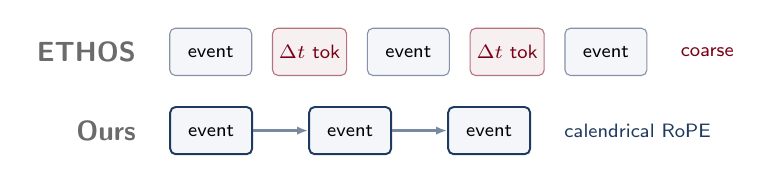
\begin{tikzpicture}[
    font=\scriptsize,
    ev/.style={draw=accent!55, fill=boxbg, rounded corners=2pt, inner sep=2pt, minimum height=6mm, text width=9mm, align=center},
    dt/.style={draw=crimson!55, fill=crimson!6, rounded corners=2pt, inner sep=2pt, minimum height=6mm, text width=8mm, align=center, text=crimson},
    lane/.style={font=\bfseries, text=muted, anchor=east},
    ar/.style={-{Latex[length=1.4mm]}, accent!60, thick}
  ]
    \node[lane] (el) at (0,1) {ETHOS};
    \node[ev, right=3mm of el] (e1) {event};
    \node[dt, right=2.5mm of e1] (d1) {$\Delta t$ tok};
    \node[ev, right=2.5mm of d1] (e2) {event};
    \node[dt, right=2.5mm of e2] (d2) {$\Delta t$ tok};
    \node[ev, right=2.5mm of d2] (e3) {event};
    \node[right=3mm of e3, text=crimson] {coarse};
    \node[lane] (ml) at (0,0) {Ours};
    \node[ev, right=3mm of ml, draw=accent, line width=0.7pt] (m1) {event};
    \node[ev, right=7mm of m1, draw=accent, line width=0.7pt] (m2) {event};
    \node[ev, right=7mm of m2, draw=accent, line width=0.7pt] (m3) {event};
    \draw[ar] (m1)--(m2); \draw[ar] (m2)--(m3);
    \node[right=3mm of m3, text=accent] {calendrical RoPE};
  \end{tikzpicture}
  \end{center}
  \vfill
  \begin{columns}[T, onlytextwidth]
    \begin{column}{0.57\textwidth}
      \begin{itemize}\setlength{\itemsep}{5pt}
        \item \textbf{MOTOR} --- time-to-event only; \emph{no Value}; constant-hazard; ``days-since-birth'' \warn{\emph{ignores the calendar}}.
        \item \textbf{STraTS} --- continuous Time \& Value, but models only $P(V_{\text{next}})$ $\Rightarrow$ \warn{\emph{no generation}}.
        \item \textbf{ETHOS} --- \emph{interval tokens} between events $\Rightarrow$ coarse, \warn{cumulative error}, longer sequences.
      \end{itemize}
    \end{column}
    \hfill
    \begin{column}{0.39\textwidth}
      \begin{tcolorbox}[title={The gap}]
        No prior model unifies \textbf{numeric Value} $+$ \textbf{calendrical Time} $+$ \textbf{generative foreseeing} --- the space TCF fills.
      \end{tcolorbox}
    \end{column}
  \end{columns}
  \vfill
\end{frame}

% ---------------------------------------------------------------------
% Problem / setup (Figure 1)
% ---------------------------------------------------------------------
\begin{frame}{Setup: from raw EHR to a triplet token sequence}
  \framesubtitle{Figure 1. Chronological events $\to$ (T, F, V) tokens with continuous timestamps}
  \begin{columns}[t]
    \begin{column}{0.62\textwidth}
      \begin{center}
        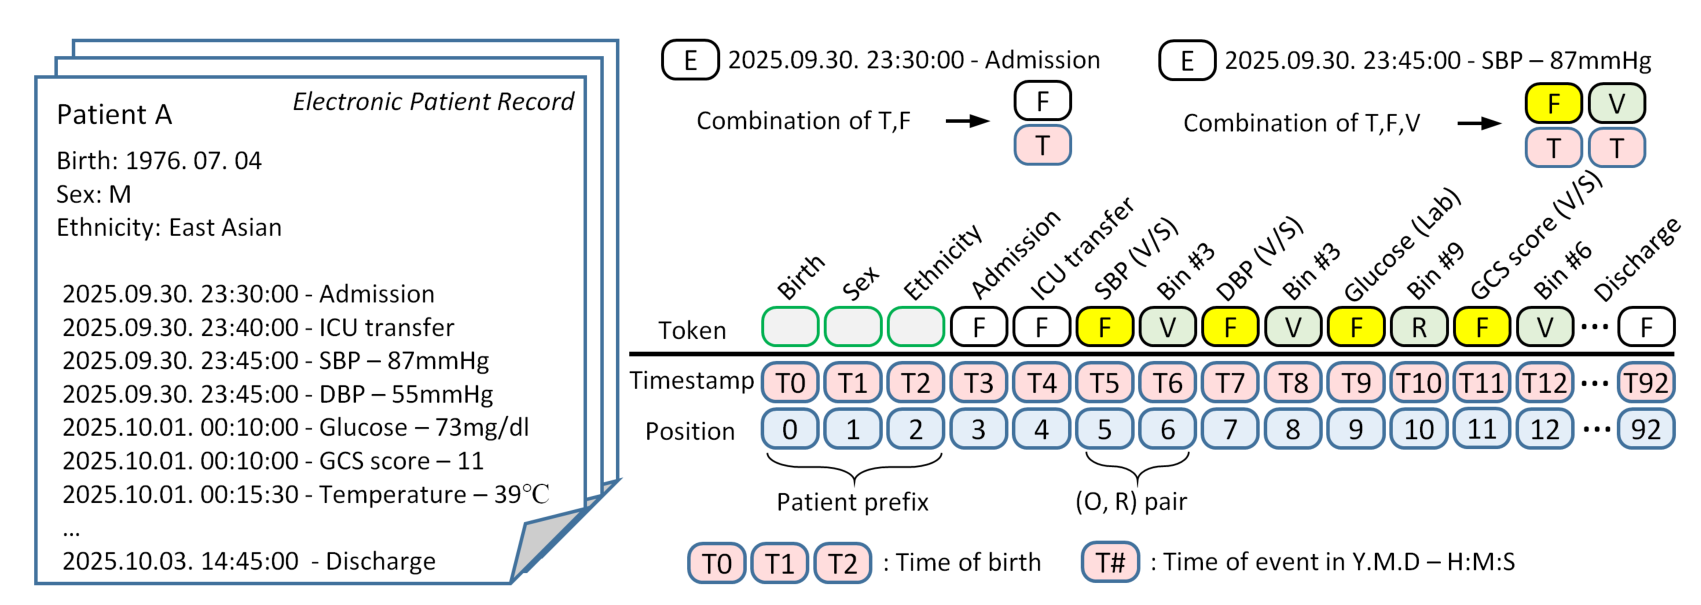
\includegraphics[width=\linewidth]{figures/fig1_tokenization.png}\\[2pt]
        \figcap{Figure 1. Patient prefix, then per-event Feature/Value tokens; timestamps stay continuous.}
      \end{center}
    \end{column}
    \begin{column}{0.38\textwidth}
      \vfill
      \begin{itemize}\setlength{\itemsep}{7pt}
        \item Each event $E$ $\to$ \textbf{Feature} token (e.g.\ SBP) $+$ \textbf{Value} token (e.g.\ 87\,mmHg).
        \item Multiple events may share \emph{one} timestamp (concurrent labs).
        \item \textbf{Position} disambiguates co-occurring events; \textbf{time} carries the calendar.
      \end{itemize}
      \vfill
    \end{column}
  \end{columns}
\end{frame}

% =====================================================================
\section{Method}
% =====================================================================

% ---------------------------------------------------------------------
% Problem definition & notation
% ---------------------------------------------------------------------
\begin{frame}{Problem definition \& notation}
  \framesubtitle{Autoregressive generative modeling over (Time, Feature, Value) event tokens}
  \vfill
  \begin{columns}[T, onlytextwidth]
    \begin{column}{0.46\textwidth}
      \begin{itemize}\setlength{\itemsep}{6pt}
        \item \textbf{Input} --- patient $=$ chronological events $E_{1:L}$, each $E_k=(T_k,F_k,V_k)$.
        \item \textbf{Tokens} --- event $\to$ \emph{Feature} token $+$ binned \emph{Value} token; timestamp $T_k$ stays \good{\emph{continuous}} (drives RoPE).
        \item \textbf{Pretrain} --- autoregressive over the token stream; learn the next event \emph{and} its timing.
      \end{itemize}
      \smallskip
      \begin{tcolorbox}[title={Learning objective}]
        NTP \warn{models only} $P(F_{\text{next}}\!\mid\! E_{\text{past}})$. TCF adds \emph{time}:
        \[ P(T_{\text{next}}\!\mid\! E_{\text{past}}),\;\; P(F_{\text{fore}}\!\mid\! T_{\text{fore}}, E_{\text{past}}). \]
      \end{tcolorbox}
    \end{column}
    \hfill
    \begin{column}{0.48\textwidth}
      \scriptsize
      \renewcommand{\arraystretch}{1.25}
      \setlength{\tabcolsep}{5pt}
      \begin{tabular}{@{}r @{\ \ } >{\raggedright\arraybackslash}p{0.74\textwidth}@{}}
        \toprule
        \multicolumn{2}{@{}l}{\textbf{Notation}}\\
        \midrule
        $E_k$ & $k$-th event $=(T_k,F_k,V_k)$\\
        $T_k$ & continuous timestamp (calendrical)\\
        $F_k$ & feature (e.g.\ SBP, lab code)\\
        $V_k$ & numeric value $\to$ binned token\\
        $\rho,\,w$ & KDE density \& inverse-density weight\\
        $d$ & model dim, split $d_{\text{pos}}{+}d_{\text{time}}$ (24{+}40 of 64)\\
        $s_j$ & calendrical period (min, hour, day\ldots)\\
        $\Delta T_{\text{n}}$ & interval to the next event\\
        $\Delta T_{\text{f}}$ & horizon(s) to forecast\\
        $h_{\text{last}}$ & last hidden state\\
        $\mathcal{L}$ & TCF loss $=L_{\text{next time}}{+}L_{\text{fore}}$\\
        \bottomrule
      \end{tabular}
    \end{column}
  \end{columns}
  \vfill
\end{frame}

% ---------------------------------------------------------------------
% Method overview (Figure 2)
% ---------------------------------------------------------------------
\begin{frame}{Method overview: three EHR-native components}
  \framesubtitle{Figure 2. (A) Pathology-Focused Binning \textperiodcentered{} (B) Dual-Calendar RoPE \textperiodcentered{} (C) TCF objective}
  \vfill
  \begin{center}
    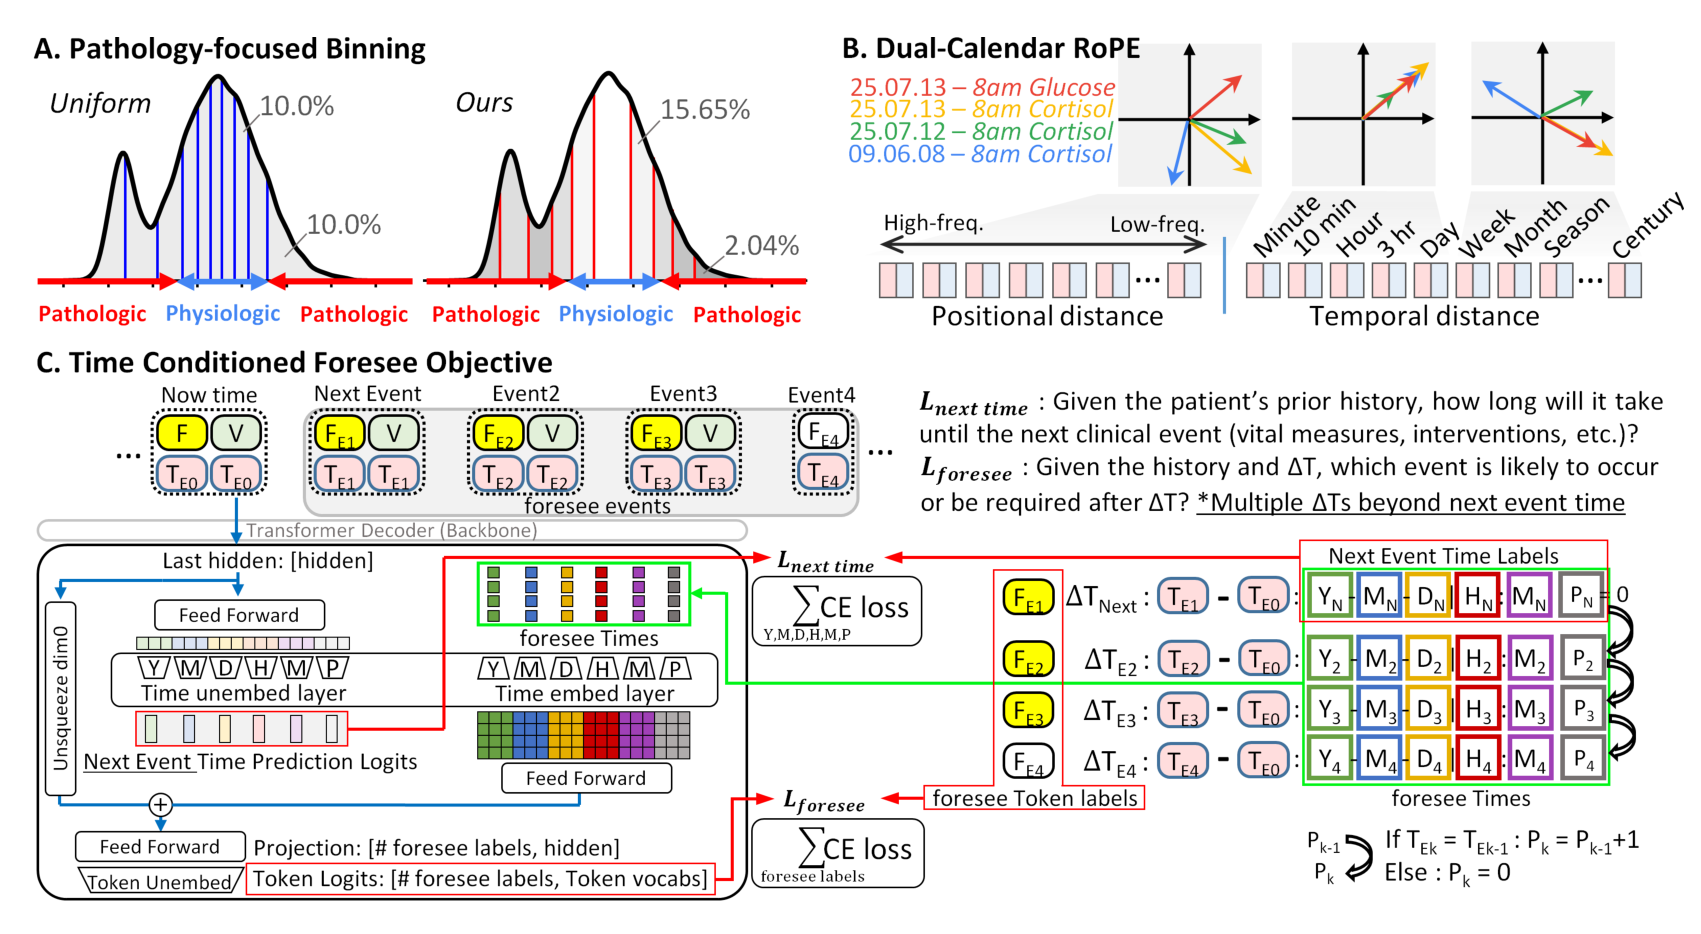
\includegraphics[width=0.86\linewidth]{figures/fig2_method.png}\\[3pt]
    \figcap{Figure 2. A: \good{density-based bins} favor pathologic ranges. B: position vs.\ calendrical time. C: $L_{\text{next time}} + L_{\text{foresee}}$.}
  \end{center}
  \vfill
\end{frame}

% ---------------------------------------------------------------------
% (1) Pathology-Focused Binning
% ---------------------------------------------------------------------
\begin{frame}{(1) Pathology-Focused Binning}
  \framesubtitle{Spend resolution where it is clinically decisive --- the abnormal tails}
  \vfill
  \begin{columns}[T]
    \begin{column}{0.54\textwidth}
      \begin{itemize}\setlength{\itemsep}{7pt}
        \item \textbf{KDE density}, non-parametric --- no Gaussianity assumption (\good{robust} to long tails, dual peaks).
        \item \textbf{Inverse-density weight} --- sparse \warn{\emph{pathologic}} values weighted up, dense \emph{normal} values down.
        \item \textbf{Weighted percentile bins} --- finer partition in clinically important ranges.
        \item First to bring density-adjusted binning to EHR FMs.
      \end{itemize}
    \end{column}
    \begin{column}{0.46\textwidth}
      \begin{tcolorbox}[title={KDE density \& weight}]
        \[ \rho(x_k)=\sum_{j=1}^{|V^f_{\text{list}}|} K_h(x_k - v_j) \]
        \[ K_h(u)=\exp\!\Big(\!-\tfrac{u^2}{2(0.1\sigma)^2}\Big) \]
        \[ w(v)\propto \rho(v)^{-N},\quad N\ge 1 \]
        \centering{\figcap{weighted count $c'_j = c_j\cdot w(v_j)$}}
      \end{tcolorbox}
    \end{column}
  \end{columns}
  \vfill
\end{frame}

% ---------------------------------------------------------------------
% (2) Dual-Calendar RoPE
% ---------------------------------------------------------------------
\begin{frame}{(2) Dual-Calendar RoPE}
  \framesubtitle{Split the RoPE dimensions: token order $\Vert$ calendrical clock}
  \vfill
  \begin{columns}[T]
    \begin{column}{0.54\textwidth}
      \begin{itemize}\setlength{\itemsep}{7pt}
        \item Partition $x=[x_{\text{pos}}\Vert x_{\text{time}}]$, $d=d_{\text{pos}}+d_{\text{time}}$ \;(24 + 40 of 64).
        \item \textbf{Positional} part --- truncated RoPE; orders \good{\emph{co-occurring}} events at the same timestamp.
        \item \textbf{Temporal} part --- phase within \good{calendrical periods} (minute, hour, day, month\ldots).
        \item Encodes ``same test, same hour, different day'' \& event concurrency.
      \end{itemize}
    \end{column}
    \begin{column}{0.46\textwidth}
      \begin{tcolorbox}[title={Rotation angles}]
        \[ \theta^{(\text{pos})}_{p,i}=\frac{p}{10000^{2i/d}} \]
        \[ \theta^{(\text{time})}_{t,j}=\Big(\frac{t \bmod s_j}{s_j}\Big)\cdot 2\pi \]
        \centering{\figcap{$q'=[\mathrm{RoPE}(q_{\text{pos}},\theta^{(\text{pos})})\Vert \mathrm{RoPE}(q_{\text{time}},\theta^{(\text{time})})]$}}
      \end{tcolorbox}
    \end{column}
  \end{columns}
  \vfill
\end{frame}

% ---------------------------------------------------------------------
% (3) TCF objective
% ---------------------------------------------------------------------
\begin{frame}{(3) Time-Conditioned Foreseeing (TCF)}
  \framesubtitle{Predict \emph{when}, then forecast \emph{what} across multiple future horizons}
  \vfill
  \begin{columns}[T]
    \begin{column}{0.5\textwidth}
      \begin{itemize}\setlength{\itemsep}{7pt}
        \item NTP models only $P(F_{\text{next}}\!\mid\! E_{\text{past}})$ --- \warn{time-blind}.
        \item \textbf{$L_{\text{next time}}$} --- predict $\Delta T_{\text{next}}$ as a calendrical vector (10-yr $\to$ 1-min), CE over $N_{\text{scales}}$.
        \item \textbf{$L_{\text{foresee}}$} --- re-inject future $\Delta T_{\text{foresee}}$, fuse with $h_{\text{last}}$, \good{forecast events} at those times.
        \item Mirrors clinical \good{\emph{planning}}: ``what is needed in the next 6\,h?''
      \end{itemize}
    \end{column}
    \begin{column}{0.5\textwidth}
      \begin{tcolorbox}[title={TCF objective}]
        \[ h_{\text{conditioned}}=\mathrm{FFN}\big(\mathrm{LN}(h_{\text{last}}+\mathrm{FFN}(e_{\text{time}}))\big) \]
        \[ \mathcal{L}=L_{\text{next time}} + L_{\text{foresee}} \]
        \centering{\figcap{learns $P(T_{\text{next}}\!\mid\! E_{\text{past}})$ \emph{and} $P(F_{\text{foresee}}\!\mid\! T_{\text{foresee}}, E_{\text{past}})$}}
      \end{tcolorbox}
      \smallskip
      \figcap{Value modeling: same form with $\Delta T\!=\!0$, conditioned on the current Feature.}
    \end{column}
  \end{columns}
  \vfill
\end{frame}

% =====================================================================
\section{Experiments}
% =====================================================================

% ---------------------------------------------------------------------
% Experimental setup
% ---------------------------------------------------------------------
\begin{frame}{Setup: MIMIC-III benchmark, reproduced baselines}
  \framesubtitle{Tables 2--3. Public data, open code; all baselines re-run under identical backbone}
  \vfill
  \begin{center}
  \renewcommand{\arraystretch}{1.4}
  \setlength{\tabcolsep}{5pt}
  \begin{tabular}{@{}>{\bfseries}l p{0.70\textwidth}@{}}
    \toprule
    \normalfont\textbf{Component} & \textbf{Setup}\\
    \midrule
    Data & MIMIC-III v1.4 \textperiodcentered{} Harutyunyan split \textperiodcentered{} 28.7k/5.1k patients \textperiodcentered{} 38.6M events\\
    Configs & 3 feature sets: \textbf{117} (all), \textbf{17} (vitals), \textbf{6} (core vitals)\\
    Tasks (7) & IHM, Phe, Dec-death, Dec-arrest, LOS, HUO, Vaso\\
    Metrics & AUROC, AUPRC (binary) \textperiodcentered{} macro-F1, Cohen's $\kappa$ (multiclass)\\
    Baselines (8) & HEART, MOTOR, EHRSHOT, TRADE, EHRmamba (no-share); FM4EHR, ETHOS, STraTS (share)\\
    Backbone & Transformer decoder \textperiodcentered{} 64-dim K/Q (24 pos + 40 time) \textperiodcentered{} ctx 2048\\
    \bottomrule
  \end{tabular}
  \end{center}
  \vfill
  \figcap{\;\;Ours evaluated \emph{with} and \emph{without} value sharing; each compared to its \good{matched baseline group}.}
  \vfill
\end{frame}

% ---------------------------------------------------------------------
% Main results (Table 3)
% ---------------------------------------------------------------------
\begin{frame}{Main results: \#1 on every task, both value modes}
  \framesubtitle{Table 3. 117-feature config --- AUROC / AUPRC etc.\ (test loss for 117/17/6 at left)}
  \begin{center}
  \scriptsize
  \renewcommand{\arraystretch}{1.05}
  \setlength{\tabcolsep}{2.6pt}
  \begin{tabular}{l ccc cc cc cc cc cc cc cc}
    \toprule
    & \multicolumn{3}{c}{\textbf{Test loss} $\downarrow$} & \multicolumn{2}{c}{IHM} & \multicolumn{2}{c}{Phe} & \multicolumn{2}{c}{Dec-d.} & \multicolumn{2}{c}{Dec-a.} & \multicolumn{2}{c}{LOS} & \multicolumn{2}{c}{HUO} & \multicolumn{2}{c}{Vaso}\\
    \cmidrule(lr){2-4}\cmidrule(lr){5-6}\cmidrule(lr){7-8}\cmidrule(lr){9-10}\cmidrule(lr){11-12}\cmidrule(lr){13-14}\cmidrule(lr){15-16}\cmidrule(lr){17-18}
    \textbf{Method} & 117 & 17 & 6 & ROC & PRC & maF1 & $\kappa$ & ROC & PRC & ROC & PRC & maF1 & $\kappa$ & ROC & PRC & ROC & PRC\\
    \midrule
    \multicolumn{18}{@{}l}{\itshape\color{muted} No value share}\\
    HEART     & 5.30 & 5.43 & 5.84 & .838 & .442 & .150 & .142 & .869 & .205 & .862 & .199 & .717 & .718 & .703 & .701 & .865 & .363\\
    MOTOR     & 4.95 & 5.21 & 5.65 & .872 & .547 & .174 & .163 & .904 & .272 & .889 & .261 & .770 & .773 & .753 & .748 & .891 & .438\\
    EHRSHOT   & 5.84 & 6.08 & 6.34 & .801 & .433 & .101 & .115 & .829 & .167 & .802 & .153 & .634 & .633 & .701 & .614 & .867 & .341\\
    TRADE     & 5.26 & 5.45 & 6.05 & .828 & .441 & .158 & .151 & .867 & .170 & .857 & .165 & .738 & .738 & .732 & .731 & .869 & .393\\
    EHRmamba  & 5.14 & 5.44 & 5.93 & .868 & .557 & .150 & .159 & .901 & .277 & .886 & .260 & .690 & .687 & .751 & .753 & .873 & .399\\
    \rowcolor{accent!12}
    \textbf{Ours} & \textbf{4.69} & \textbf{4.91} & \textbf{5.37} & \textbf{.889} & \textbf{.607} & \textbf{.181} & \textbf{.185} & \textbf{.928} & \textbf{.400} & \textbf{.917} & \textbf{.388} & \textbf{.809} & \textbf{.816} & \textbf{.776} & \textbf{.781} & \textbf{.912} & \textbf{.498}\\
    \midrule
    \multicolumn{18}{@{}l}{\itshape\color{muted} Value share}\\
    FM4EHR    & 6.43 & 6.39 & 6.40 & .617 & .177 & .023 & .003 & .744 & .075 & .778 & .102 & .530 & .519 & .598 & .653 & .690 & .130\\
    ETHOS     & 4.97 & 5.25 & 5.57 & .859 & .530 & .170 & .165 & .900 & .311 & .890 & .304 & .739 & .746 & .721 & .731 & .890 & .437\\
    STraTS    & 5.79 & 5.81 & 6.07 & .759 & .311 & .123 & .121 & .840 & .141 & .804 & .103 & .656 & .661 & .590 & .598 & .864 & .331\\
    \rowcolor{accent!12}
    \textbf{Ours} & \textbf{4.88} & \textbf{5.04} & \textbf{5.56} & \textbf{.876} & \textbf{.559} & \textbf{.173} & \textbf{.170} & \textbf{.910} & \textbf{.319} & \textbf{.902} & \textbf{.310} & \textbf{.781} & \textbf{.784} & \textbf{.749} & \textbf{.755} & \textbf{.906} & \textbf{.470}\\
    \bottomrule
  \end{tabular}
  \end{center}
  \vspace{1pt}
  \figcap{\;\;Dec-arrest AUPRC {\blue .388} vs MOTOR .261 ($+49\%$); Dec-death AUPRC {\blue .400} vs .277 ($+44\%$) --- \good{decisive} under 1:40 \warn{imbalance}.}
\end{frame}

% ---------------------------------------------------------------------
% AUROC curves (Figure 3)
% ---------------------------------------------------------------------
\begin{frame}{Statistically significant gains over 2nd-best}
  \framesubtitle{Figure 3. AUROC curves, Ours vs.\ MOTOR, 95\% CI via bootstrap}
  \begin{columns}[t]
    \begin{column}{0.68\textwidth}
      \begin{center}
        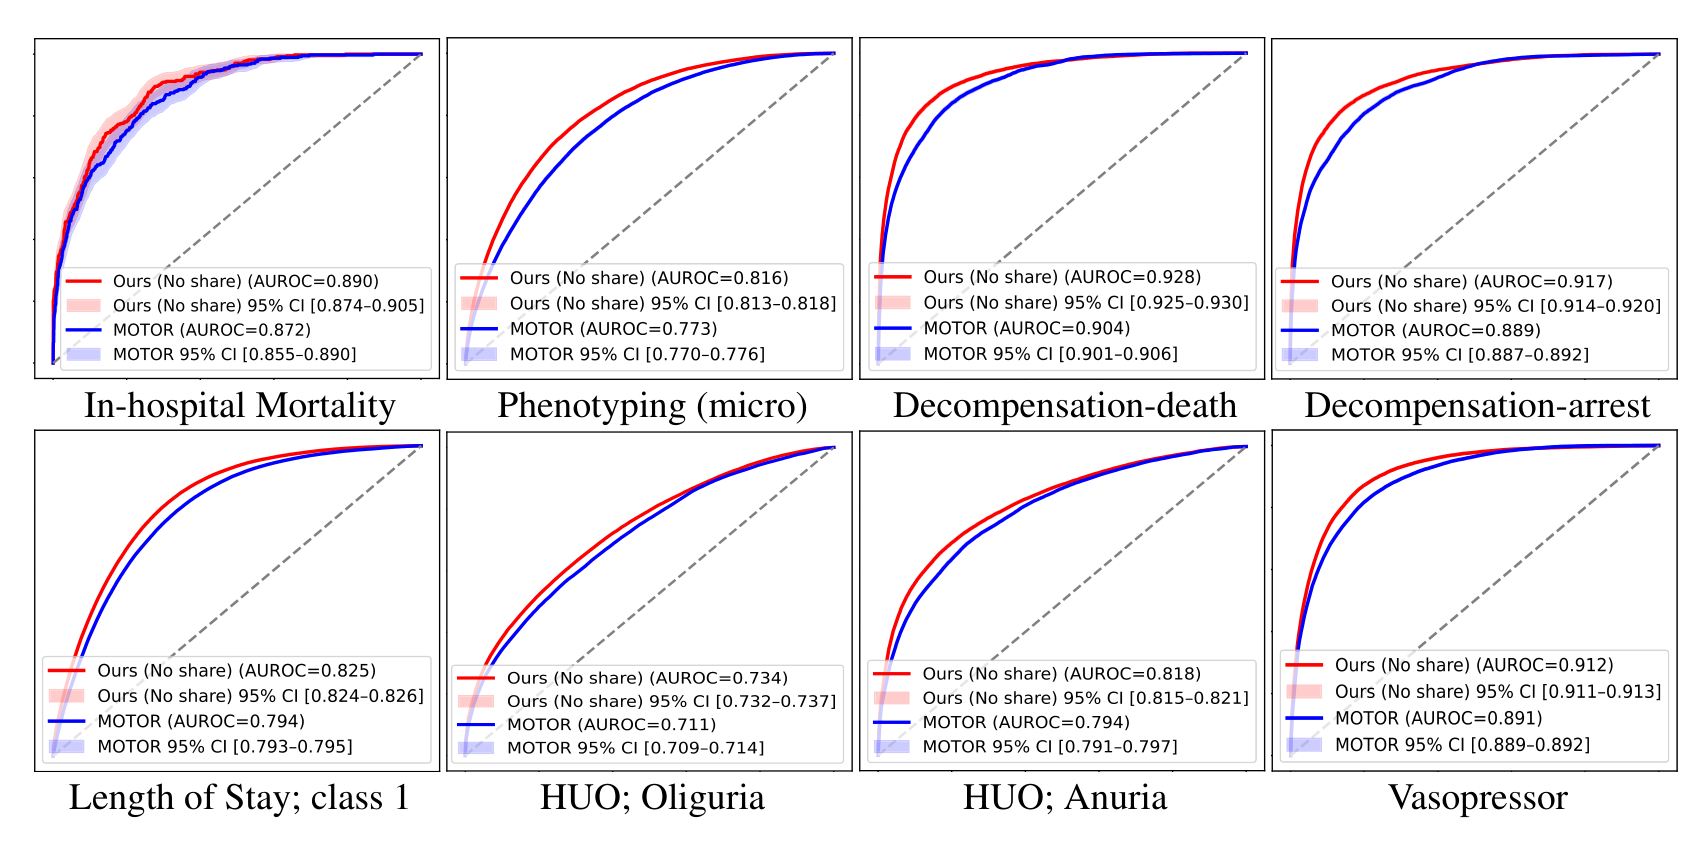
\includegraphics[width=\linewidth]{figures/fig3_auroc.png}\\[2pt]
        \figcap{Figure 3. 7 tasks (LOS as binary class-1; Phe micro-ROC; HUO split oliguria/anuria).}
      \end{center}
    \end{column}
    \begin{column}{0.32\textwidth}
      \vfill
      \begin{itemize}\setlength{\itemsep}{10pt}
        \item Ours (blue) \good{dominates} MOTOR (red) on \emph{every} task.
        \item Non-overlapping CIs $\Rightarrow$ significant.
        \item IHM .890 vs .872 \textperiodcentered{} Dec-death .928 vs .904.
      \end{itemize}
      \vfill
    \end{column}
  \end{columns}
\end{frame}

% ---------------------------------------------------------------------
% Ablation (Table 4)
% ---------------------------------------------------------------------
\begin{frame}{Ablation: every component pulls its weight}
  \framesubtitle{Table 4. Strip components back to a plain NTP transformer (117-feature test loss)}
  \vfill
  \begin{columns}[c]
    \begin{column}{0.52\textwidth}
      \centering
      \renewcommand{\arraystretch}{1.35}
      \setlength{\tabcolsep}{6pt}
      \begin{tabular}{l l l c}
        \toprule
        \textbf{Binning} & \textbf{Embedding} & \textbf{Objective} & \textbf{Test loss} $\downarrow$\\
        \midrule
        \rowcolor{accent!12}
        Pathology & Dual-Cal.\ & TCF & \textbf{4.686}\\
        Uniform   & Dual-Cal.\ & TCF & 4.713\\
        Uniform   & RoPE       & TCF & 4.810\\
        Uniform   & RoPE       & NTP & 5.241\\
        \bottomrule
      \end{tabular}
    \end{column}
    \begin{column}{0.48\textwidth}
      \begin{itemize}\setlength{\itemsep}{12pt}
        \item \textbf{TCF $\to$ NTP} is the largest drop ($-0.43$): \good{the objective matters most}.
        \item \textbf{Dual-Calendar RoPE} adds $\approx 0.10$ over plain RoPE.
        \item \textbf{Pathology binning} trims a further $0.03$.
        \item All three \good{stack monotonically}.
      \end{itemize}
    \end{column}
  \end{columns}
  \vfill
\end{frame}

% ---------------------------------------------------------------------
% Generation quality (Figure 4 textual) + human/LLM eval (Figure 5)
% ---------------------------------------------------------------------
\begin{frame}{Generation quality: consistent, realistic trajectories}
  \framesubtitle{Figures 4--5. Given an initial record, forecast the continued medical history}
  \vfill
  \begin{columns}[T]
    \begin{column}{0.55\textwidth}
      \begin{tcolorbox}[title={Content \& temporal consistency}]
        \begin{itemize}\setlength{\itemsep}{4pt}
          \item GCS $=$ E$+$V$+$M --- Ours respects it; ETHOS \warn{violates} (E2/V1/M5; GCS3).
          \item Ours emits early \emph{emergency labs} $\to$ routine vitals; ETHOS emits \emph{no labs}.
          \item Ours: dense tests at admission $\to$ \emph{hourly} routine; ETHOS irregular.
        \end{itemize}
      \end{tcolorbox}
    \end{column}
    \begin{column}{0.45\textwidth}
      \begin{tcolorbox}[title={Human \& LLM evaluation (Fig.\ 5)}]
        \begin{itemize}\setlength{\itemsep}{4pt}
          \item 100 generated samples per group.
          \item 5 physicians \textperiodcentered{} 5 non-medical \textperiodcentered{} 4 LLMs.
          \item Ours \good{\emph{preferred over ETHOS}} across all groups.
        \end{itemize}
      \end{tcolorbox}
    \end{column}
  \end{columns}
  \vfill
\end{frame}

% ---------------------------------------------------------------------
% Calendrical analysis (Figure 6)
% ---------------------------------------------------------------------
\begin{frame}{Calendrical generation: day--night physiology emerges}
  \framesubtitle{Figure 6. Vital signs generated across a 24-h window, averaged over 1{,}000 samples}
  \begin{columns}[t]
    \begin{column}{0.62\textwidth}
      \begin{center}
        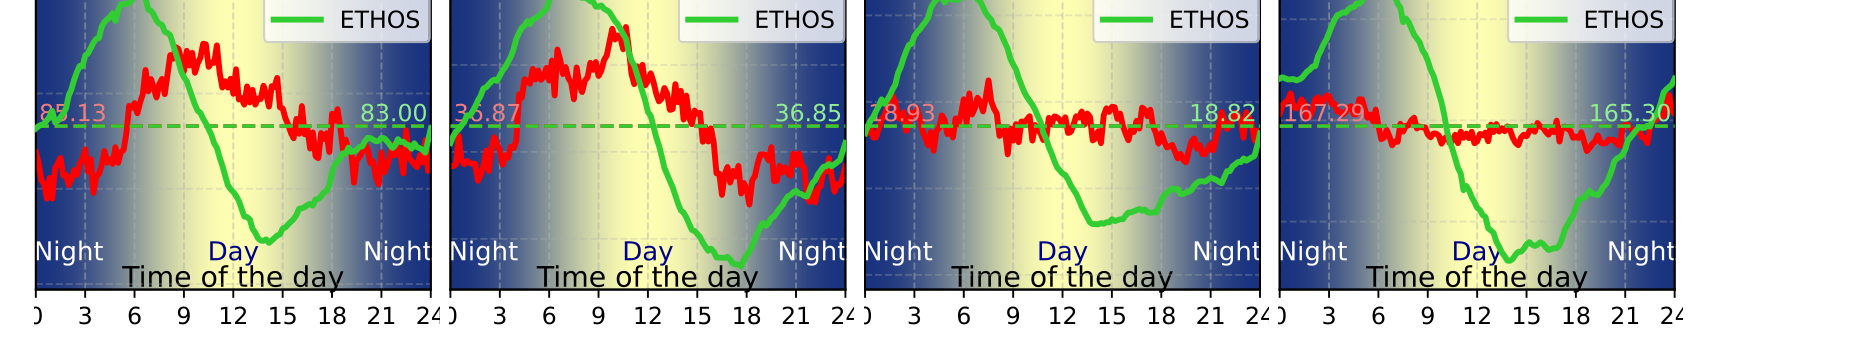
\includegraphics[width=\linewidth]{figures/fig6_calendrical.png}\\[3pt]
        \figcap{Figure 6. Ours (green) vs.\ ETHOS (red): HR/temp/RR higher by day; Height (control) flat.}
      \end{center}
    \end{column}
    \begin{column}{0.38\textwidth}
      \vfill
      \begin{itemize}\setlength{\itemsep}{9pt}
        \item Ours \good{reproduces} \textbf{circadian} rise in HR, temperature, respiratory rate.
        \item Height (control) stays \emph{flat} --- no spurious rhythm.
        \item ETHOS: \warn{\emph{implausible}} patterns even on the control.
      \end{itemize}
      \vfill
    \end{column}
  \end{columns}
\end{frame}

% =====================================================================
\section{Takeaways}
% =====================================================================

% ---------------------------------------------------------------------
% Limitations
% ---------------------------------------------------------------------
\begin{frame}{Limitations}
  \framesubtitle{Honest gaps the paper itself flags}
  \vfill
  \begin{itemize}\setlength{\itemsep}{14pt}
    \item \textbf{No generation metric} --- \warn{no established quantitative measure} for \emph{temporal} EHR generation; timing-appropriateness is hard to score, so generation is judged only qualitatively / by human \& LLM preference.
    \item \textbf{Single dataset} --- validated on \warn{MIMIC-III only}; cross-institution / cross-EHR transfer untested.
    \item \textbf{Hand-set calendrical periods} --- predefined unit set (minute$\to$10-yr) and RoPE dim split (24/40) are design choices, not learned.
  \end{itemize}
  \vfill
  \begin{tcolorbox}[title={Open direction}]
    Developing quantitative \emph{temporal-generation} metrics is called out as key future work for EHR foundation models.
  \end{tcolorbox}
  \vfill
\end{frame}

% ---------------------------------------------------------------------
% Takeaways
% ---------------------------------------------------------------------
\begin{frame}{Takeaways}
  \vfill
  \begin{itemize}\setlength{\itemsep}{16pt}
    \item {\large\bfseries\blue Design for EHR, not NL} \;—\; binning, positions, and objective each \good{re-tuned to EHR structure} $\to$ \#1 on all 3 configs $\times$ 7 tasks.
    \item {\large\bfseries\blue Time is first-class} \;—\; Dual-Calendar RoPE $+$ TCF capture \warn{irregular intervals} \emph{and} calendrical rhythm; AUPRC up to {\hl +48\%}.
    \item {\large\bfseries\blue Genuine temporal generation} \;—\; \good{first EHR model} to forecast \emph{time-conditioned} events with realistic circadian dynamics.
  \end{itemize}
  \vfill
  \begin{tcolorbox}[title={Medical-AI implication}]
    Pathology-aware, time-conditioned pretraining is a strong foundation for \emph{long-range clinical forecasting} --- deploy as decision \emph{support} with human review.
  \end{tcolorbox}
  \vfill
\end{frame}

% ---------------------------------------------------------------------
% References
% ---------------------------------------------------------------------
\begin{frame}{References}
  \small
  \begin{thebibliography}{9}
    \bibitem{tcf} Kang, B.\,G.\ et al.\ \emph{Time-Conditioned Foreseeing: Temporal Generative Pretraining for EHR Foundation Models}. ICML, 2026.
    \bibitem{strats} Tipirneni, S.\ \& Reddy, C.\,K.\ \emph{Self-Supervised Transformer for Sparse and Irregularly Sampled Multivariate Clinical Time-Series (STraTS)}. ACM TKDD, 2022.
    \bibitem{motor} Steinberg, E.\ et al.\ \emph{MOTOR: A Time-to-Event Foundation Model for Structured Medical Records}. ICLR, 2024.
    \bibitem{ethos} Renc, P.\ et al.\ \emph{Zero-Shot Health Trajectory Prediction Using Transformer (ETHOS)}. npj Digital Medicine, 2024.
    \bibitem{rope} Su, J.\ et al.\ \emph{RoFormer: Enhanced Transformer with Rotary Position Embedding}. Neurocomputing, 2024.
    \bibitem{mimic} Harutyunyan, H.\ et al.\ \emph{Multitask Learning and Benchmarking with Clinical Time Series Data (MIMIC-III)}. Scientific Data, 2019.
  \end{thebibliography}
\end{frame}

\end{document}
